% Reviewed until Home Status Displays \subsection{Reminder <to be specified>}
% (see additional remark below)

Following our exploration of the smart home and connected car last quarter, the team branched out to a broader design space to dig deeper into compelling technology and customer needs.
\section{Extended Benchmarking}
\label{sec:benchmarking}

During the early benchmarking phase last quarter, we got familiar with the following concepts:

\begin{itemize}
    \item The future of smart cars
    \item Everything that makes up a modern Audi of today
    \item An overview of the current status of smart home technology
    \item Existing connections between home and car
\end{itemize}

\noindent
In summary, we found that smart home technology on the market today offers convenience to users such as the ability to monitor their home from anywhere and remotely control lights from their smart phone, however many users are deterred by the complexity of setup, lack of security, questionable reliability, and obsolescence of such devices. Previous benchmarking details can be found under Appendix \ref{sec:benchmarkingAppendix} and in our fall report.

\subsection{Is 2016 the Year of the Smart Home?}
%As much as 2016 is the year of Linux on the desktop *scnr*

% {Jonathan} Agreed, this is benchmarking. Will move it.
%\todo{Johanna: Not sure if the following subsection belongs here. We did not do needfinding there, it is facts from surveys done by others so rather some kind of benchmarking I would say. If you look at last year's needfinding section it really was compact and short and only summarized all the needs they found in the fall and winter quarter and directly leads on to their final prototype. + This section and the "from needs to prototypes"-section I wrote have some overlaps, we should try and merge that\\
%Dylan: I agree there's some overlap, and I think that's okay. I see from needs to prototypes as being an overall implications of what our results found, and so to me it's okay as is.}

During the last quarter, we mainly explored the technological side of smart homes. This quarter, we were particularly interested in adoption of smart home technology and predictions of future adoption. Despite the technical hurdles to consumer adoption of smart home technology, the belief persists that smart home technology will become ever more ubiquitous. Coldwell Banker conducted a survey of US consumers, and made the following claims:
\begin{itemize}
\item 45\% of users own or will adopt smart home technology in 2016.
\item 70\% of people said buying one smart home product made them want to buy another.
\item The top choices for a home to be considered "smart" were:
    \subitem Locks and alarms (63\%)
    \subitem Temperature (63\%)
    \subitem Light bulbs and lighting systems (58\%)
    \subitem Safety such as fire and CO detectors (56\%)
\item Adopters were slightly more male (57\%) and more likely to be millennials than any other demographic (43\%)
\end{itemize}

\noindent
This defines what has been called the "first wave" of smart home technology. One key distinction for their definition of "smart" is that it includes entertainment systems such as TVs with internet connectivity which are not included in our definition of smart home.

The 2015 State of the Smart Home Report by Icontrol Networks mirrors many of the same findings as the Coldwell Banker report, though adding that "simplicity and ease-of-use trump technological innovation - and today's consumers want devices that solve real, everyday problems" and "right now, most consumers see smart home as a nebulous term without a clear value proposition." This is essentially what our benchmarking and needfinding culminated to last quarter, and has presented significant challenges to our design development. The smart home space offers intriguing features and ample opportunity, but does not address significant latent needs of consumers, yet.

\noindent
Two unique nuggets from the Smart Home Report are:
\begin{itemize}
    \item 72\% of users would sleep better if their parents had smart technology that could alert them if there was a problem.
    \item Insurers are subsidizing and investing in smart technology so that users feel the company is taking a more proactive role in their lives and security, instead of just waiting for an incident to occur. [citation http://fortune.com/2015/12/09/smart-home-insurance/]
\end{itemize}

\noindent
The first point emphasizes security and monitoring as the perceived main driver for smart home adoption. While the primary generation of smart home adopters, millenials, are not as convinced by that need, as their Baby Boomer parents age, the worry about health and safety increases.

The second point offers an interesting avenue to substantially increase smart home technology adoptions, if one was interested in pursuing it. If smart technology can (1) increase the visibility and trust in  companies or (2) reduce potential liability of an incident for insurance companies, then they will be highly motivated to encourage users to adopt smart home technology. Many users do not necessarily have high opinions of their insurance companies, and one representative mentioned that 90\% of users never file a claim, so how can insurance companies still benefit users? This begs the question of how a car company like Audi might benefit users with encouraging adoption of some smart technology that could lower their car insurance premiums such as through more active car monitoring and theft prevention. If our eventual system was able to give users tangible reductions in insurance premiums, both Audi and consumers would be more interested in adopting the technology. And as the Coldwell Banker survey found, having one smart home product makes people want to buy more, so it would also be in the best interest of smart home companies like SmartThings and Wink to encourage any and all adoption of smart home products.

Most of all, users want simplicity and do not want any additional complexity in their lives, even if they have the time, resources, and ability to set up smart devices. They do not want to waste money on products, particularly hardware for their home, if it may be obsolete in a few years. When replacing light switches, one could spend 8X as much for a smart switch that connects to Wink in comparison to a traditional one, but smart technology does not yet offer that much value to consumers. If a system fails, the user may not know how to fix it. One user's convenience is another's inconvenience.

We cannot know for sure if or when smart home technology will become ubiquitous, but we do know that systems that maximize on the user experience and offer significant value to consumers will have the greatest chance at success. Technological innovation for the sake of innovation is not enough to satisfy consumers. So many other aspects of our technologically driven lives are designed with a smooth user experience in mind, and smart home technology cannot be any different. Decades ago, users would put up with pain points in the interface of early email or mobile telephones because of the value it added to their lives, but smart home technology does not currently add such revolutionary capability.

\subsection{Traditional Home Security Systems}

With security being the most important aspect for a smart home, we wanted to get a better understanding of traditional home security systems and their smart home counterparts. Traditionally monitored home security systems have been around for decades through companies such as ADT and Brinks. Users have sensors, control panels, cameras, etc. professionally installed, and then pay a subscription to have a company monitor their home and contact the authorities if the alarm is triggered. Users manually arm system upon departure by pressing a button on the keypad, and must enter a code upon arrival home within a short time to avoid activating alarm. 

\begin{figure}[ht]
\centering
	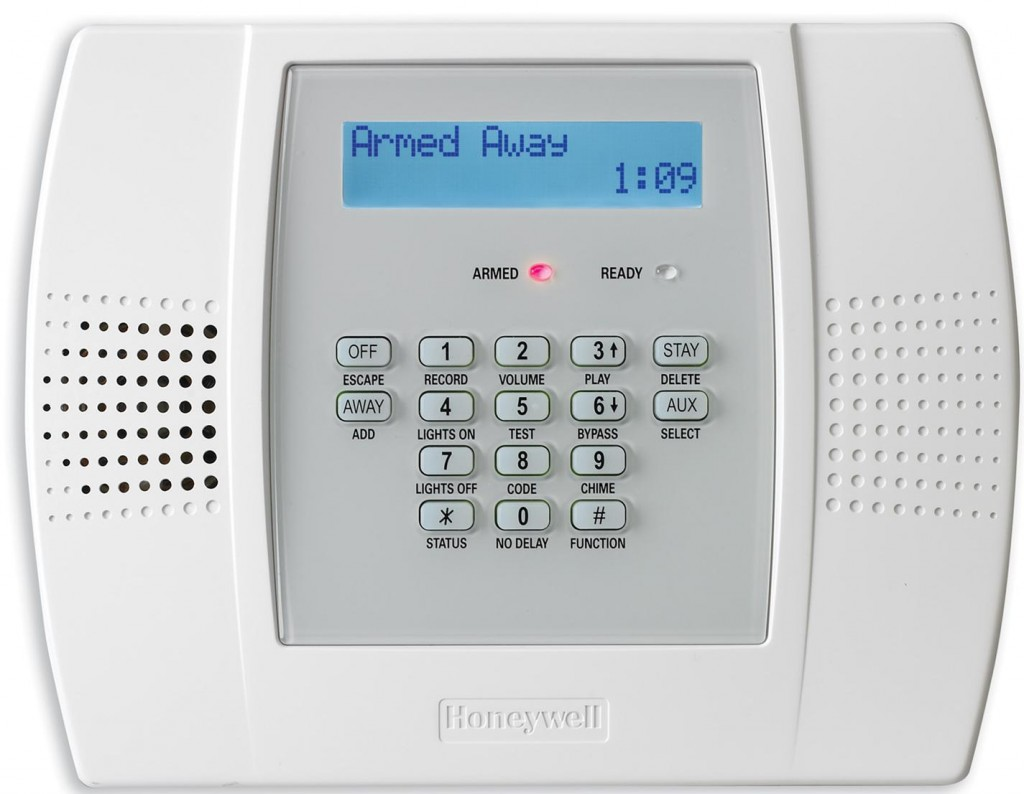
\includegraphics[keepaspectratio, width=4in]{Figures/Benchmarking/keypad.jpg}
	\caption{Sample traditional home security interface. Users must enter code in order to disarm system to avoid false alarm. \protect\footnotemark}
	\label{fig:keypad.jpg}
\end{figure}

\footnotetext{Taken from \url{http://zionssecurity.com/faq-security/the-top-15-questions-about-adt-home-security-systems/} on March 17th 2016}

One noticeable problem with such systems is false alarms, which cost the US economy an estimated \$1.8 billion per year \cite{Blackstone2007}. Users may forget to disable the security system upon entry, or it may be inadvertently set off by babysitters, housekeepers, or pets. Users may be fined for each incident that police unnecessarily respond to, with rising fees for each incident in the same year \cite{Blackstone2007}. Consequently, some users report owning and paying for systems but not often turning them on, to avoid the worry of false alarms. This leaves the home at risk for break-ins.

Of more recent evolution is the idea of full home security and automation, primarily motivated by cable companies trying to shift into another market as traditional cable subscriptions wane. Companies like Comcast, Time Warner, and AT\&{}T offer customers the option to have security systems installed and monitored along with what would be considered the first wave of smart home technology: lights, thermostats, and cameras that can be monitored from anywhere with an Internet connection. Traditional home security companies are now in this space as well, offering higher levels of home automation than before. The advantage of these systems is that they are set up by professionals, avoiding the large complex learning curve that limits adoption of existing add-on smart home technology.

More advanced home security systems today offer users the ability to monitor cameras in the home remotely and arm and disarm the security system at a distance with an additional key fob. In interviews with users, we found that they do not often use the remote monitoring feature, assuming that if there's a problem, the alarm will go off.

Remote key fob disarming presents serious security risks, even with encrypted rolling code sequences. Car thefts occur every year because thieves capture codes when users are parked and lock or unlock their cars. In 2015, a serious flaw in the security of car smart key systems, including Audi/VW, was published by Samy Kamkar \cite[pp. 58 -- 67]{CarKeyHack}.
%\todo{Jonathan: I discovered another hack that sounds simpler. Hope you're ok with it? It's also referenced in the article you provided a link to. Also, I think there's no need to go into too much detail here. Cars can be hacked using their key fobs as a message should be enough.
Potential hackers could intercept the transmission between a user's key fob and car twice, reducing the potential billions of codes down to approximately 200,000, small enough that the code could be guessed by a computer within half an hour.

This could be accomplished using inexpensive and readily available hardware. If the same technology is used in homes, they would be at greater risk as they are stationary, while cars are mobile. A thief could hide electronics to capture wireless codes in the home owner's front entryway, capturing the necessary information to prepare for a future break-in.
%\todo{Jonathan: Same as above, this section should not be concerned with our idea yet
As such, we must be mindful of the potential hackability of our system in the future.
%\todo{Jonathan: I think the citation of the car hack I provided above is a bit better since it is a lot simpler for users of the exploit} - all great, thanks - DJM
%[citation http://www.dailymail.co.uk/sciencetech/article-3201564/Hackers-reveal-flaw-100-cars-kept-secret-Volkwagen-TWO-YEARS-Bug-used-unlock-Kia-Lamborghini.html]

\subsection{DIY Home Security Systems in Smart Homes}

Security is the primary reason that users are interested in adopting smart home technology \cite{ABIhomeAutomationReport2015}. With the advent of modular and adaptable smart home technology, it has become easier for "do-it-yourself (DIY)" users to set up and monitor their own security systems avoiding the costly installation and subscription fees of traditional home monitoring companies. They offer peace of mind at a reasonable cost. All-in-one systems such as Canary\footnote{Canary Connect, Inc. (\url{https://canary.is})}(\ref{fig:canary.jpg} offer motion detection, cameras, and alarms, and will alert user if trouble is detected, but will not call authorities directly, reducing the response time in the event of a true emergency. As a result, these systems do not necessarily have the same magnitude of trouble with costly false alarms as traditional systems, but also do not deter theft as much as more actively monitored systems. There is an obvious trade-off between functionality and cost. \cite{DIYSecurity}

\begin{figure}[ht]
\centering
	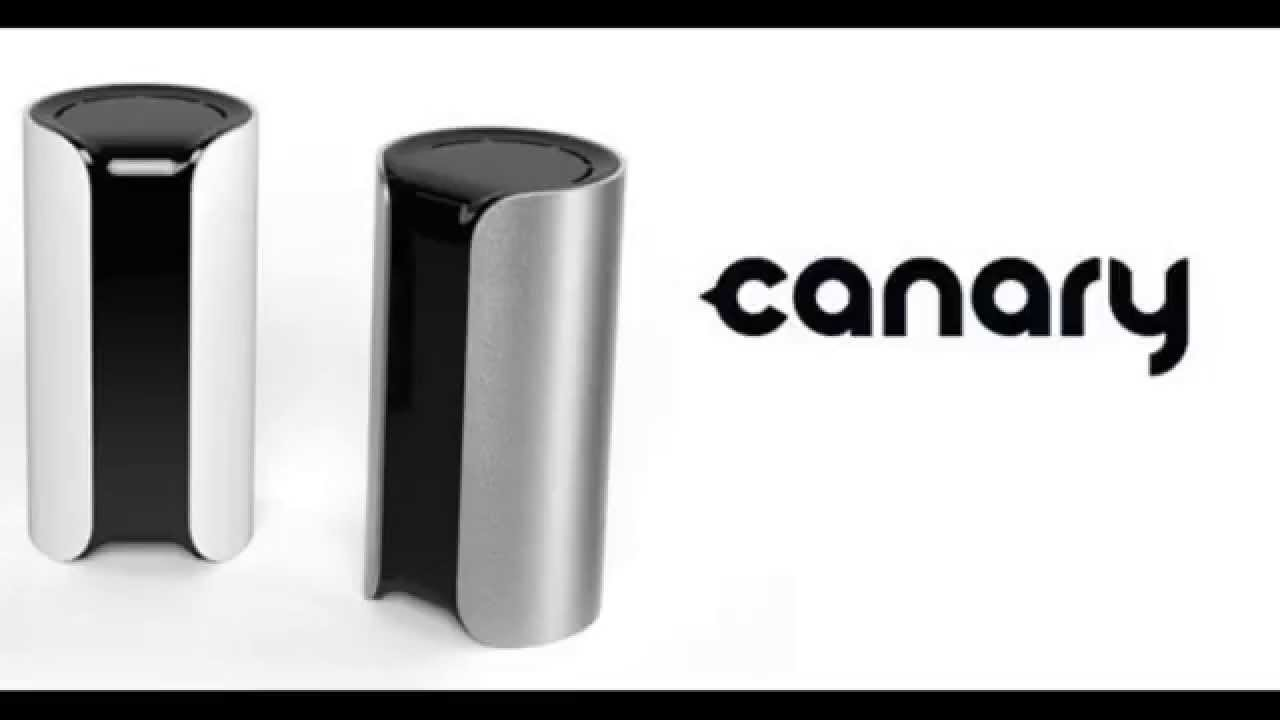
\includegraphics[keepaspectratio, width=6in]{Figures/Benchmarking/canary.jpg}
	\caption{Canary smart home security system allows users to monitor their home from their smart phone. Canary alerts users if significant motion is detected and helps users to contact authorities if intruder is detected. Online storage of video helps users to record and review suspicious moments throughout the day. \protect\footnotemark}
	\label{fig:canary.jpg}
\end{figure}
\footnotetext{Taken from \url{https://www.youtube.com/watch?v=DJUVWkmrqVQ} on March 17th 2016}

\subsection{Smart Locks}

One of the most exciting, but often disappointing, smart home security technologies is the idea of a smart door lock that can be activated remotely with a user's smart phone. This allows one to give temporary "keys" to guests who can let themselves into a user's home using their phone or allow the user to open the front door remotely if there is a package delivery. These locks, such as August\footnote{August Home, Inc. (\url{http://august.com})} (see figure \ref{fig:august.jpg}) advertise the ability to lock and unlock automatically as the user leaves or arrives home. However, the reliability of such systems is questionable, and at least one user we interviewed expressed serious security concerns with such systems. However, another user we interviewed, an architect for high end homes, said that smart locks are becoming quite common in homes, as users want the ability to let others in throughout the day such as babysitters, housekeepers, and mailmen.

Whereas the potential of such systems is exciting, the implementation issues and security risks limit adoption. We can assume that these issues may diminish substantially in the next few years. Moreover, many of the professional home security services described above offer users the ability to remotely lock and unlock their front doors, and as third-party systems become more stable, adoption will likely increase significantly. The last thing users want to do after a long day at work and commute is fumble with their keys in the dark outside their home, and the idea of eliminating that step smooths the user's transition into and away from home significantly.

\begin{figure}[ht]
\centering
	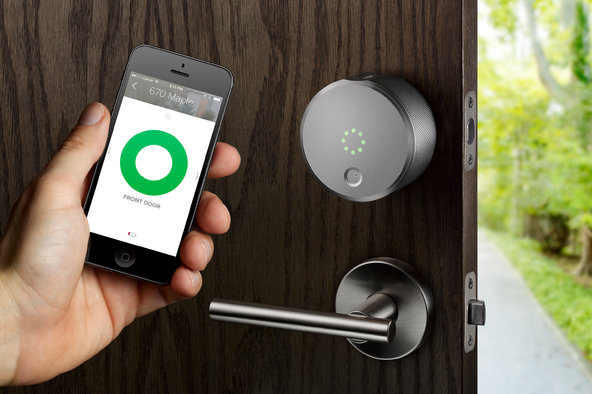
\includegraphics[keepaspectratio, width=6in]{Figures/Benchmarking/august.jpg}
	\caption{August smart lock for the front door can be activated from a user's smart phone. Temporary digital "keys" can be given to visitors so that remote access can be granted while homeowner is away. \protect\footnotemark}
	\label{fig:august.jpg}
\end{figure}
\footnotetext{Taken from \url{http://bits.blogs.nytimes.com/2014/10/14/the-august-smartlock-shows-why-you-should-stick-with-dumb-keys} on March 17th 2016}

\subsection{Home Status Displays} 
%martin
With smart homes having more and more sensors and controllable elements arises the question on how to keep the user in control or convey the status to them. There are several different systems available.

Almost every smart home device or system comes with a smart phone app for control and status functionality. These apps usually have a dashboard-like screen showing the current state of the appliances as well as possibilities to switch devices and configure more complex settings. Figure \ref{fig:wink_relay} shows an example of a smart light bulb control interface. These applications allow users to check on and control the smart home from their phones.

\begin{figure}[ht]
\centering
	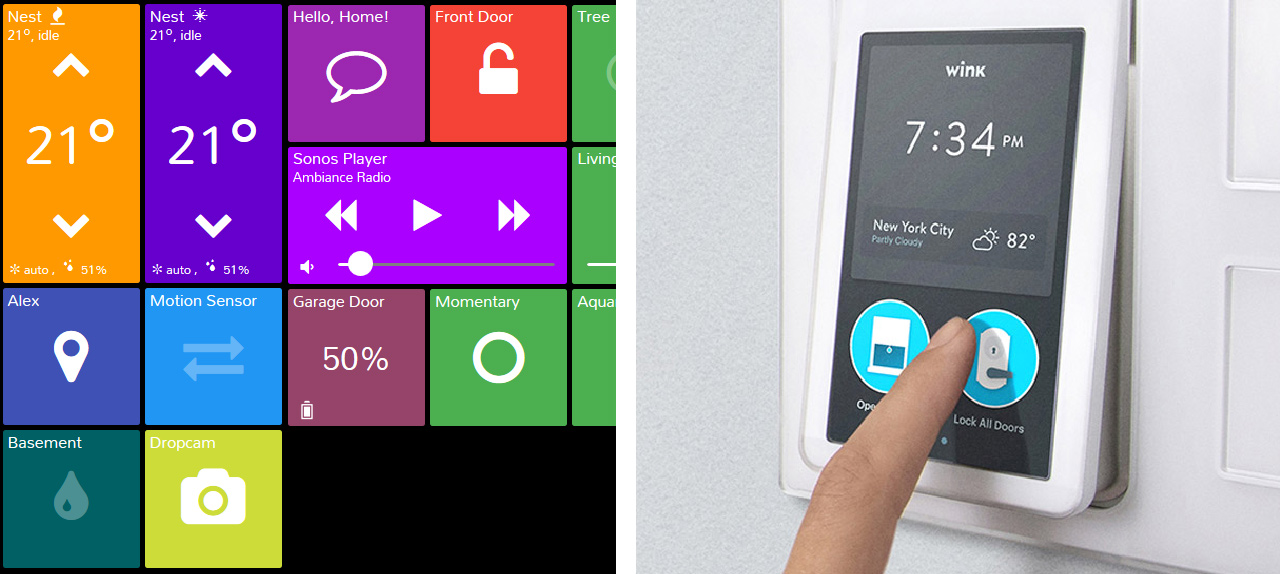
\includegraphics[keepaspectratio, width=6in]{Figures/Benchmarking/wink_smarttiles.jpg}
	\caption{On the left is an example dashboard of the SmartTiles webapp. The image on the right shows the Wink Relay.}
	\label{fig:wink_relay}
\end{figure}

Another category of status displays are bigger dashboards that are installed at a central spot. These usually are dedicated devices for the purpose of interacting with the smart home. Figure \ref{fig:wink_relay} shows the Wink Relay as well as the SmartTiles web app. Both serve as central control and information interface with slightly different approaches. While the Wink Relay uses single purpose hardware the SmartTiles solution relies on existing devices such as tablets or screens that home owners can mount to a wall. These dashboard systems vary widely in features, format, customizability and interaction possibilities.

\begin{figure}[ht]
\centering
	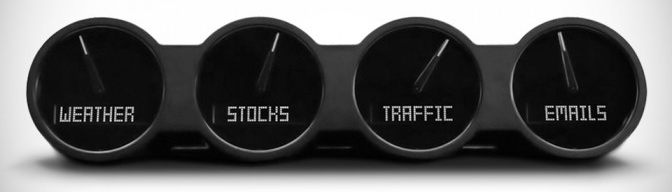
\includegraphics[keepaspectratio, width=5in]{Figures/Benchmarking/quirky_gauge.jpg}
	\caption{The Quirky Nimbus, an analogue gauge displaying various information.\protect\footnotemark}
	\label{fig:quirky_gauge}
\end{figure}

\footnotetext{Taken from \url{http://ecx.images-amazon.com/images/I/41JbtXXjyDL._SY355_.jpg} on March 12th 2016}

\subsection{Reminders and Locators} 
%martin
There are different methods available to aid users not to forget or lose things. Similar to the analog to-do lists there are applications serving the same purpose with added functionality. These apps can notify users by various means (visual, audible, tactile) at specified dates or intervals or when entering or leaving designated areas (geofencing). 

\begin{figure}[ht]
\centering
	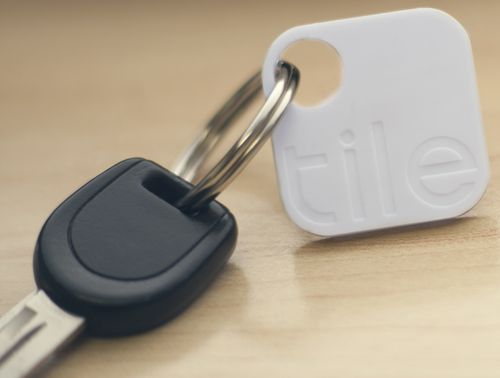
\includegraphics[keepaspectratio, width=3in]{Figures/Benchmarking/Tile_tag.jpg}
	\caption{A Tile bluetooth tag attached to a key.\protect\footnotemark}
	\label{fig:tile}
\end{figure}

\footnotetext{Taken from \url{http://www.rfidjournal.com/lib/x/a/assets/2013/08/Tile_tag.jpg} on March 16th 2016}

With the current Bluetooth Smart (Bluetooth Low Energy) specification a new class of products emerged to aid people locate things. These are small tags that can be attached to important objects. These tags can then be located by means of a smart phone application. The app can determine the distance to the tag up to a range of 30m. Because of the low energy consumption of the radio module, they can run up to a year on a single, small battery. Most tags can also make a noise or vibrate on request from the app. An exemplary product is the Tile tag\cite{tile} displayed in Figure \ref{fig:tile}.

Further applications of this technology include small dedicated buttons that can be attached where the user likes and either are freely programmable or have a fixed purpose.
The Flic smart button\cite{flic} is an example of the first kind, easily programmable by integrating the IFTTT service (for explanation of this see Appendix \ref{text:ifttt}). 
There are more products that add functionality, for example motion, heat and volume sensors into these small buttons like the Sen.se peanuts\cite{peanuts}. These allow the user to add smart features to objects of her everyday life.

Every item users want to be reminded of needs to have a tag attached if it does not have some sort of radio communication itself (e.g. cloth, documents etc.). The Bluetooth tag technology described above is still too expensive and energy consuming for use cases such as sports cloths. There are passive radio-frequency identification tags available which only activate through power delivered from a reader device nearby. These tags can be very cheap and thus can be imagined to be attached to everyday objects\cite{weis2007rfid}. Hsu et al. have described a system that attaches such passive tags to a users items. Based on the users history and calendar information it will then remind her about objects to bring along when leaving his home\cite{hsu2011rfid}.

\subsection{Car Status}
There are a number of ways to get status information about the car from a distance.

The open standard for On-board diagnostics data (OBD) makes a vast veriety of the car's paramaters easily accessible. It has been mandatory to built this into every new car for a number of years. However, it gained widespread popularity only since recently a number of silicon valley tech startups have been using adapters to wirelessly transmit this data to the users' smartphones to generate value for their customers. 

Car manufcaturer have started to make specific functionalities of their models be controllable via smartphone apps. For example, the AudiConnect smartphone app allows users to lock/unlock their car remotely and keep tabs of where the driver parked.

Another example is the Nissan Leaf App which offers a broad set of functionalities like monitoring the battery charge level (Figure~\ref{fig:NissanLeaf1}) and checking on the car's inside temperature as well as adjusting the air conditioning settings (Figure~\ref{fig:NissanLeaf2}).

\begin{figure}[h]
\centering
	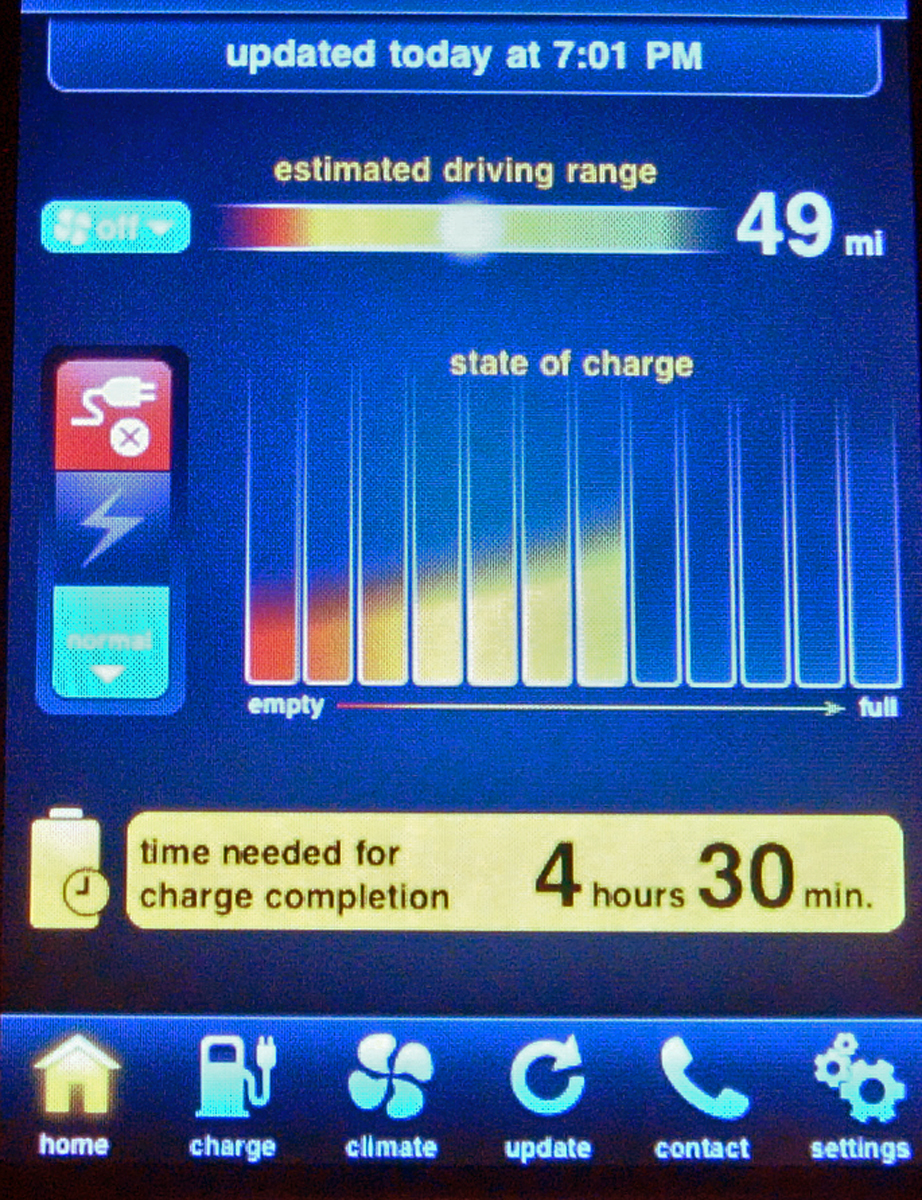
\includegraphics[keepaspectratio, width=3in]{Figures/Nissan_Leaf_mobile_app_battery_status_1733.jpg}
	\caption{Nissan Leaf smart phone app for EV status showing: driving range left, state of charge and time required to complete a full charge.\protect\footnotemark}
	\label{fig:NissanLeaf1}
\end{figure}

\footnotetext{Taken from \url{https://commons.wikimedia.org/wiki/File:Nissan_Leaf_mobile_app_battery_status_1733.jpg} on March 17th 2016 (CC BY-SA 2.0)}

\begin{figure}[h]
\centering
	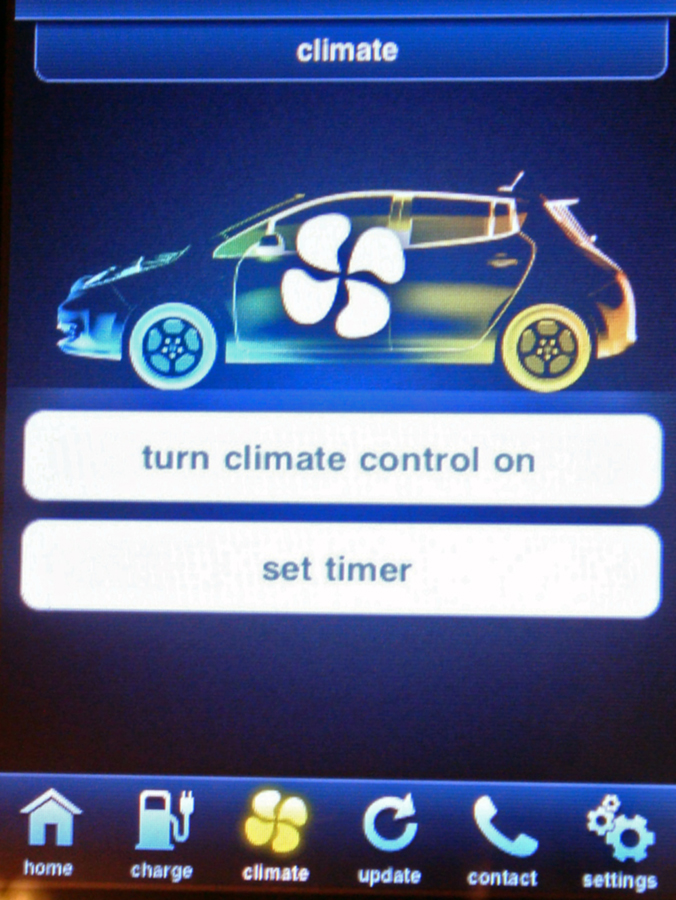
\includegraphics[keepaspectratio, width=3in]{Figures/Nissan_Leaf_mobile_app_climate_control_1713.jpg}
	\caption{Nissan Leaf smart phone app to turn on remotely the climate control.\protect\footnotemark}
	\label{fig:NissanLeaf2}
\end{figure}

\footnotetext{Taken from \url{https://commons.wikimedia.org/wiki/File:Nissan_Leaf_mobile_app_climate_control_1713.jpg} on March 17th 2016 (CC BY-SA 2.0)}

\subsection{Small Modular displays}
%jonas
Since electronic components have become smaller and smaller, certain research groups experimented with the possibilities of very small computers with very small displays.
Siftables (Figure \ref{fig:siftables}) have been designed almost ten years ago. They are small artifacts that can display information and sense certain aspects about their environment. They are connected with other computers through a wireless interface.~\cite{Merrill:2007:STS:1226969.1226984}

\begin{figure}[ht]
\centering
	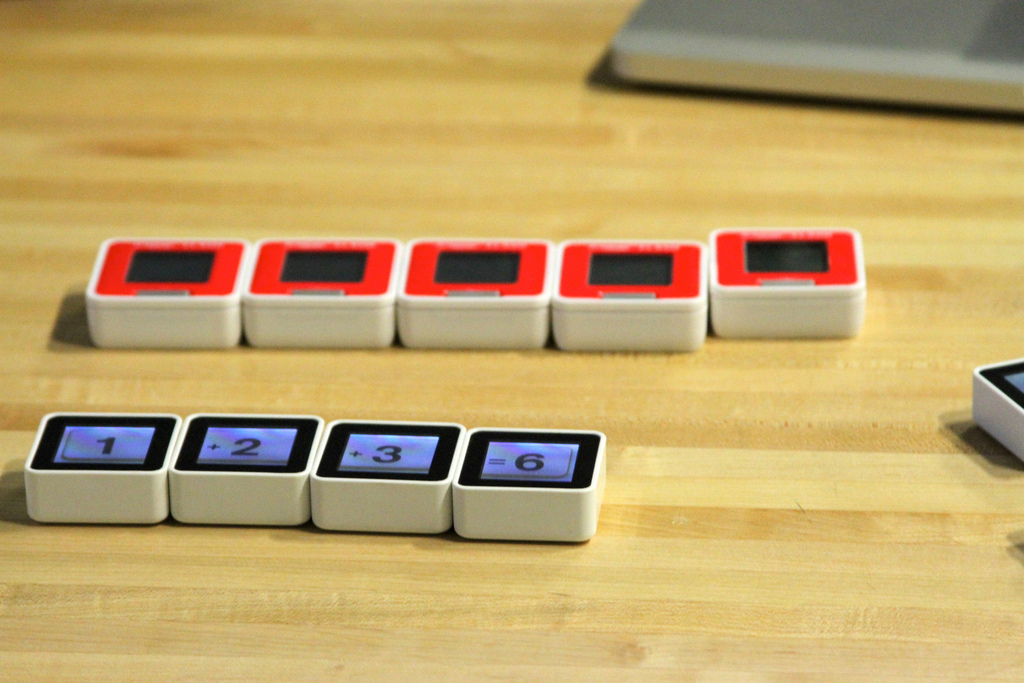
\includegraphics[keepaspectratio, width=6in]{Figures/siftables.jpg}
	\caption{Siftables lined up displaying pieces of information.\protect\footnotemark}
	\label{fig:siftables}
\end{figure}


\footnotetext{Taken from \url{https://www.flickr.com/photos/natematias/6244330415/} on March 12th 2016 (CC BY-SA 2.0)}

After Siftables gained viral popularity online, the company Sifteo was founded and has since then manufactured and sold so-called Sifteo Cubes. After limited financial success of the product, most of its software is now open-source.~\footnote{http://venturebeat.com/2014/12/23/sifteos-intelligent-cubes-go-open-source-after-disappointing-commercial-run/ - accessed  on March 12th 2016}

In 2015 the CloudDrops project (Figure \ref{fig:clouddrops}) followed a similar approach. These devices are supposed to display in particular web-based information and are designed to fit into more diverse architectural scenarios than Siftables.~\cite{Olberding:2015:CSP:2757710.2757718}

The Nimbus by Quirky (Figure \ref{fig:quirky_gauge}) is a recent, but unsuccessful, attempt at displaying basic information through simple displays. This made information available such as weather, travel time to chosen destination given traffic (e.g. work) at any given time. Users found the implementation poor, but did appreciate the desired functionality.

\begin{figure}[ht]
\centering
	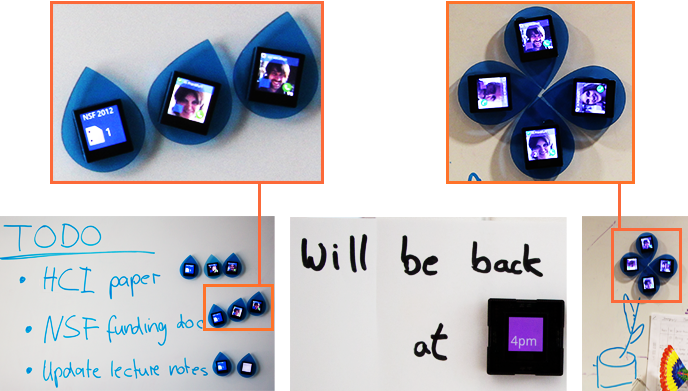
\includegraphics[keepaspectratio, width=6in]{Figures/clouddrops.png}
	\caption{Clouddrops in different usage scenarios.\protect\footnotemark}
	\label{fig:clouddrops}
\end{figure}

\footnotetext{Taken from \url{https://embodied.mpi-inf.mpg.de/research/clouddrops/} on March 12th 2016}

For certain applications, Electronic Paper technology could be an interesting choice --- Especially when displays are supposed to survive long stretches of time without being charged. Small displays using this technology are available at a pricepoint around \$33.~\protect\footnote{https://www.adafruit.com/products/1347 - accessed on March 12th 2016}.

\clearpage{}